% Master file. Compile with:  cd paper && /opt/data/bin/tectonic main.tex
%
% Structure follows the two reference papers: SKILL.state (arXiv:2608.26263)
% for the horizon-scaling presentation, Ledger (arXiv:2608.00808) for the
% deterministic execution-state framing and component ablations.
%
% EVERY NUMBER comes from paper/generated/numbers.tex, which is written by
% analysis/build_paper.py from the canonical run CSV. Do not type a measured
% number into a section file.

\documentclass[11pt,a4paper]{article}
\usepackage[margin=1in]{geometry}
% Shared preamble. Packages, house macros, and the switches that control
% which parts of the study are typeset.
%
% EXTENSION POINTS ARE MARKED WITH  %% EXTEND:
% Nothing in this file should ever contain a measured number.

\usepackage[T1]{fontenc}
\usepackage[utf8]{inputenc}
\usepackage{lmodern}
\usepackage{microtype}
\usepackage{amsmath,amssymb}
\usepackage{siunitx}
\sisetup{group-separator={,},detect-all}
\usepackage{booktabs}
\usepackage{tikz}
\usetikzlibrary{positioning,fit,calc,arrows.meta}
\usepackage{pgfplots}
\pgfplotsset{compat=1.18}
\usepackage{float}
\usepackage{algorithm}
\usepackage{algpseudocode}
\usepackage{graphicx}
\usepackage{xcolor}
\usepackage{enumitem}
\usepackage{caption}
\usepackage{subcaption}
\usepackage[hidelinks]{hyperref}
\usepackage{url}
\usepackage{xurl}
\usepackage{natbib}

%% EXTEND: switches for work that is not yet measured.
%% Flip \vtwotrue once the V-composition ladder has its full trial set; the
%% composition results section and its tables then enter the document.
%% Flip \etwotrue once the schema x protocol matrix (E2) has run.
\newif\ifvtwo   \vtwofalse
\newif\ifetwo   \etwofalse

%% EXTEND: draft notes. \draftnotestrue shows them, false hides them for
%% submission. They never carry a claim, only an instruction to the authors.
\newif\ifdraftnotes \draftnotestrue
\newcommand{\note}[1]{\ifdraftnotes\textcolor{red}{\small[\textbf{NOTE:} #1]}\fi}
\newcommand{\pending}[1]{\ifdraftnotes\textcolor{blue}{\small[\textbf{PENDING:} #1]}\fi}

% Source tags. Every factual statement about our own system carries one, so a
% reader can tell a measurement from a design intention without trusting prose.
\newcommand{\live}{\textsuperscript{\textsf{\scriptsize live}}}
\newcommand{\code}{\textsuperscript{\textsf{\scriptsize code}}}
\newcommand{\origin}{\textsuperscript{\textsf{\scriptsize orig}}}

% Condition names, defined once so a rename cannot desynchronise the text from
% the generated tables.
\newcommand{\Control}{\textsc{control}}
\newcommand{\StateOnly}{\textsc{state-only}}
\newcommand{\StateK}[1]{\textsc{state}$+#1$}
\newcommand{\SkillState}{\textsc{skill.state}}
\newcommand{\Ledger}{\textsc{ledger}}

% The tail parameter, referred to often enough to deserve one spelling.
\newcommand{\tailk}{k}

\newcommand{\rqref}[1]{\textbf{RQ#1}}

\captionsetup{font=small,labelfont=bf}
\setlist{itemsep=2pt,topsep=3pt}


\input{generated/numbers}

\title{\bfseries Bounded Context Is Not Bounded Information:\\
Structured State Memory Trades Capability for Prompt Size\\
in Long-Horizon Coding Agents}

\author{%
  \note{authors and affiliation pending owner decision}%
}
\date{Draft \today}

\begin{document}
\maketitle

\begin{abstract}
Structured state offers a way to bound a coding agent's active context
without carrying its full interaction history. Whether this also reduces
the cost of solving tasks depends on what the replacement memory preserves.
We evaluate SKILL.state-inspired context policies on Terminal-Bench,
varying state ownership, retained evidence, recent history, update protocol,
and schema. Model-written state reduces the median peak-prompt ratio to
\ModelStatePeakRatio{} on shared successes, yet raises the cost ratio to
\ModelStateCostRatio{} and lowers overall task success from
\ModelControlRate\% to \ModelStateRate\%. An exploratory comparison of
hybrid memory, which separates runtime records from model-written
interpretation, associates richer execution records with better success
and lower overhead than file references alone. Further enrichment does
not remove the full-history deficit. Retaining recent interactions gives
the clearest recovery: model-written and hybrid policies reach
\ModelHistorySixRate\% and \HybridHistorySixRate\%, against their respective
controls of \ModelControlRate\% and \HybridControlRate\%. The economic
outcomes differ: cost per observed success falls below the control for
model-written memory but remains above it for the hybrid variant.
The tested schema and protocol changes do not produce comparable recovery.
These results support evaluating structured memory through the evidence
it retains and the work needed to finish a task, rather than compression
alone. Recent-history retention is a measured partial remedy; the
incremental benefit of state over the same history window remains open.
\end{abstract}


\section{Introduction}
\label{sec:introduction}

A coding agent accumulates evidence as it works. A command exposes a
dependency, an edit changes the meaning of an earlier observation, and a
test rules out a proposed fix. An interaction transcript preserves these
events together with their context. Replacing that transcript with compact
state requires deciding which information later decisions will need.
The consequences extend beyond the length of the next prompt.

SKILL.state makes this replacement an explicit runtime
design~\citep{skillstate2026}. Persistent instructions, mutable structured
state, and the current observation replace an expanding conversation.
The attraction is clear: when those inputs are bounded, context need not
grow with the trajectory. But a bound on context is not a bound on the
work required to solve the task. A smaller representation may omit evidence,
require additional state-writing output, or change how the agent acts and
stops. Cache-aware pricing further separates prompt size from monetary cost.

We study this tension in a terminal-based coding agent. The evaluation
transfers the state-based runtime idea to a different model, agent, and
benchmark; it is not a reproduction of the original study. Our central
question is what information must survive history replacement for
compression to remain useful over a complete task.

The comparisons separate decisions that are easily conflated under
agent memory. First, who writes the memory? A model can maintain a
semantic account of its work, while the runtime can retain observed tool
events directly. This motivates hybrid state: execution records and
model-written interpretation have different owners. Second, what does the
runtime retain? File references, modifications, command outcomes, and
diagnostics convey different amounts of execution evidence. Third, which
original interactions remain available? A recent-history window preserves
detail without requiring the state writer to anticipate its relevance.
Finally, the update protocol and schema determine how the model expresses
its semantic memory.

The results connect these design choices to task success and resource use.
Model-written state substantially reduces peak prompts while lowering
success and increasing conditional successful-execution cost. An
exploratory component comparison shows why hybrid memory cannot be treated
as a single intervention: richer execution records perform better than
file references alone, but additional records do not yield continuous
improvement. Retaining recent interactions produces the clearest recovery
in both state families. The tested schema and protocol changes do not.

These findings motivate evaluating structured state together with its
retained evidence and surrounding history. We distinguish partial recovery from a complete
replacement for history, and separate measured results from proposed
adaptive switching or archival retrieval. The practical outcome is a set
of quality--cost trade-offs, not a universal recommendation to discard or
retain every transcript.

\section{Background}
\label{sec:background}

\subsection{Structured state memory}

\SkillState{}~\citep{skillstate2026} maintains a persistent structured state
$\Sigma_t$ and assembles each prompt as
\[
  \text{prompt}_t \;=\; [\,\text{task spec}\,] \;+\; [\,\Sigma_t\,] \;+\;
  [\,o_t\,],
\]
where $o_t$ is the latest observation and the interaction history is thrown
away. In one generation the model emits its reasoning, a state patch and an
action, $(R_t, \Delta\Sigma_t, a_t)$, as a single JSON object with exactly
the two keys \texttt{state\_patch} and \texttt{action}\origin. The runtime
checks each patch against a schema and rejects invalid ones with a
rollback-retry cycle. Schemas are written once per domain; across 100
InterCode CTF instances a single five-field schema is reused\origin.

The reported evidence is a horizon sweep on a procedural generator: the
prompt stays near \num{1800} characters from $T{=}10$ to $T{=}200$ while the
baselines grow to \num{48000}, and quality is preserved or improved\origin.
The paper's own error taxonomy for open-weight models attributes
\SI{68}{\percent} of failures to premature state overwrite or deletion\origin,
a figure we return to in \S\ref{sec:composition}, because it is an argument
for moving part of the state out of the model's hands.

\subsection{Deterministic execution state}

\Ledger{}~\citep{ledger2026} sits in the opposite design corner: a record
maintained by the runtime and derived mechanically from completed
interactions: observation records, per-file and global modification
counters, normalised command records with their outcomes. It adds no model
calls and does not modify the agent. Its own ablation separates its two
mechanisms cleanly: \emph{inform} (rendering the record at the end of the
input, where it cannot disturb an append-only prefix) produces most of the
efficiency gain, while \emph{govern} (intercepting a proposed command and
reusing an earlier result) produces most of the resolution gain\origin.

The two systems are complementary rather than competing: \SkillState{} keeps
semantic state in the model, \Ledger{} keeps objective state in the runtime.
Our composition study (\S\ref{sec:composition}) varies exactly this boundary,
and we deliberately exclude \emph{govern} from it: govern changes what the
agent does, so including it would mix a large effect into the measurement of
a smaller one.

\subsection{The assumptions under test}

Stated as checkable propositions rather than criticisms:

\begin{description}[style=nextline]
\item[A1 (schema availability)] An adequate domain schema exists before
  execution. The original gives no schema-design method and reports a
  verbatim field list for only one of its four domains\origin.
\item[A2 (positive from turn one)] Maintaining state is at worst neutral
  from the first turn. The shortest horizon reported is $T{=}10$, already
  longer than a large share of real coding tasks.
\item[A3 (sufficient statistic)] Nothing discarded is ever needed again.
  The original names this as a limitation\origin{} but does not measure it.
  This is the assumption this paper falsifies.
\item[M (measurement currency)] Cumulative token count is a valid proxy for
  cost. A full-text search of the original returns zero occurrences of
  cache, billing or monetary terminology\origin.
\end{description}

A1 and A3 are properties of the method. M is a property of how the method
was evaluated, and it is the one that hides the other two: a metric that
counts logical tokens can represent neither the cache discount that rewards
an append-only prefix nor the tool calls spent re-acquiring what the prompt
no longer carries.

\subsection{The design axis this paper uses}

Instead of comparing named architectures, we hold the mechanism fixed and
vary one integer: the number $\tailk$ of most recent verbatim exchanges kept
next to the state block.
\[
  \text{prompt}_t \;=\; [\,\text{task spec}\,] \;+\;
  [\,\text{last } \tailk \text{ exchanges}\,] \;+\; [\,\Sigma_t\,]
\]
At $\tailk{=}0$ this is exactly \SkillState{} as published. As $\tailk$
grows, the configuration approaches a transcript agent. The control is not a
point on this axis (it carries no state block at all) and is always reported
separately.

This buys three things a three-arm comparison cannot buy. It removes the
arbitrary constant that an intermediate ``hybrid'' arm would introduce; it
changes the question from \emph{which architecture} to \emph{where on the
axis the optimum lies}; and it makes the shape of the dependence visible,
which is what ultimately localises the damage (\S\ref{sec:capability}).

\section{Context Policies and Update Protocols}
\label{sec:model}
Let $P$ denote task instructions, $o_t$ the current observation, and
$H_{<t}$ preceding observable messages and tool results. Full history uses
\begin{equation}
 C_t^{\mathrm{full}}=[P,H_{<t},o_t].
 \label{eq:ctx-transcript}
\end{equation}
Structured memory instead constructs
\begin{equation}
 C_t^{\mathrm{state},k}=[P,\Sigma_t,\tau_k(H_{<t}),o_t],
 \qquad \tau_0(H)=\varnothing,
 \label{eq:ctx-state}
\end{equation}
where $\tau_k$ selects available recent records and $\tau_\infty(H)=H$.
Thus $k=\infty$ retains state \emph{and} the transcript; the no-state
full-history control is a different policy (Figure~\ref{fig:architecture}).
Neither definition assumes access to hidden reasoning.
% Adapted from the repository's original two-column architecture figure.
\begin{figure}[tbp]
\centering
\resizebox{\linewidth}{!}{%
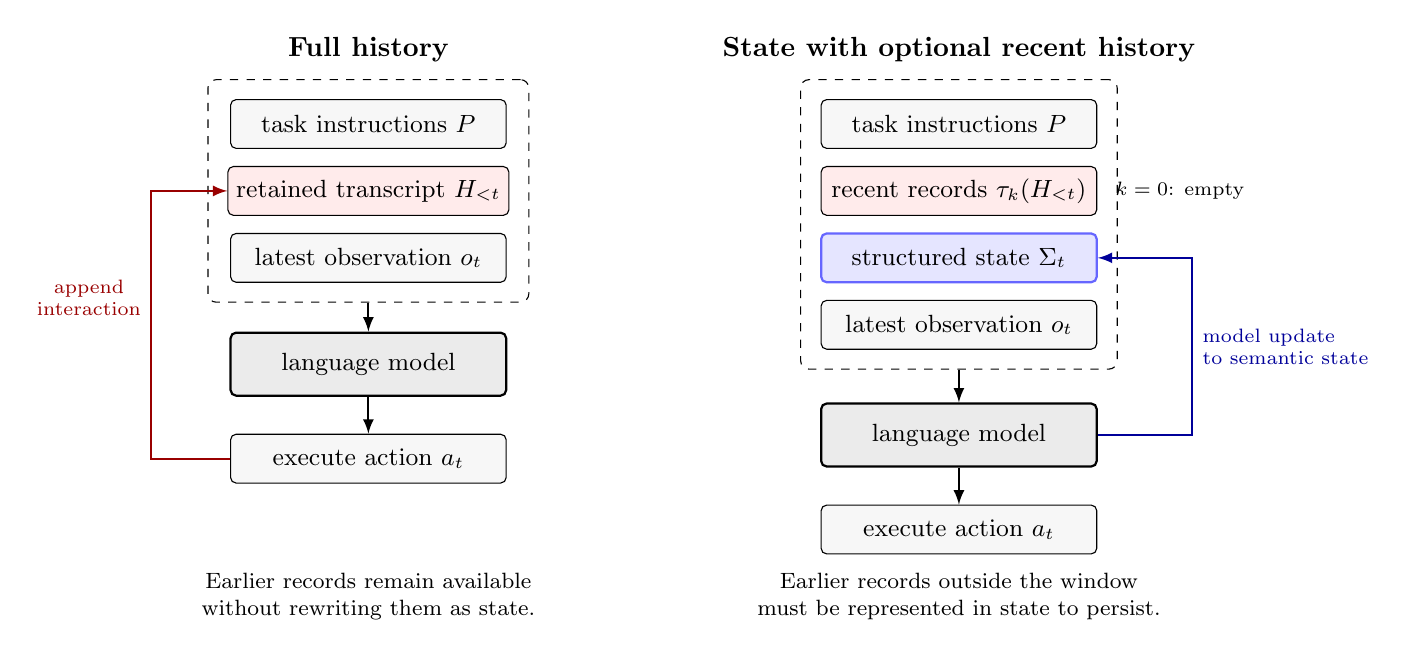
\begin{tikzpicture}[
font=\small,
box/.style={draw,rounded corners=2pt,minimum width=3.5cm,minimum height=.62cm,align=center,inner sep=3pt},
hist/.style={box,fill=red!8},
state/.style={box,fill=blue!10,draw=blue!60,thick},
plain/.style={box,fill=black!3},
llm/.style={box,fill=black!8,minimum height=.8cm,thick},
grp/.style={draw,dashed,rounded corners=3pt,inner sep=7pt},
arr/.style={-latex,thick}]
\node[font=\bfseries] at (0,4.2) {Full history};
\node[plain] (p1) at (0,3.25) {task instructions $P$};
\node[hist] (h1) at (0,2.4) {retained transcript $H_{<t}$};
\node[plain] (o1) at (0,1.55) {latest observation $o_t$};
\node[grp,fit=(p1)(h1)(o1)] (g1) {};
\node[llm] (m1) at (0,.2) {language model};
\node[plain] (a1) at (0,-1) {execute action $a_t$};
\draw[arr] (g1.south)--(m1.north);
\draw[arr] (m1)--(a1);
\draw[arr,red!60!black] (a1.west)--++(-1,0)|-(h1.west)
 node[pos=.3,left,font=\scriptsize,align=center]{append\\interaction};
\begin{scope}[xshift=7.5cm]
\node[font=\bfseries] at (0,4.2) {State with optional recent history};
\node[plain] (p2) at (0,3.25) {task instructions $P$};
\node[hist] (h2) at (0,2.4) {recent records $\tau_k(H_{<t})$};
\node[state] (s2) at (0,1.55) {structured state $\Sigma_t$};
\node[plain] (o2) at (0,.7) {latest observation $o_t$};
\node[grp,fit=(p2)(h2)(s2)(o2)] (g2) {};
\node[llm] (m2) at (0,-.7) {language model};
\node[plain] (a2) at (0,-1.9) {execute action $a_t$};
\draw[arr] (g2.south)--(m2.north);
\draw[arr] (m2)--(a2);
\draw[arr,blue!60!black] (m2.east)--++(1.2,0)|-(s2.east)
 node[pos=.25,right,font=\scriptsize,align=left]{model update\\to semantic state};
\node[right=3pt of h2,font=\scriptsize] {$k=0$: empty};
\end{scope}
\node[font=\footnotesize,align=center] at (0,-2.75) {Earlier records remain available\\without rewriting them as state.};
\node[font=\footnotesize,align=center] at (7.5,-2.75) {Earlier records outside the window\\must be represented in state to persist.};
\end{tikzpicture}}
\caption{Context policies. State replaces the older transcript, while the retention parameter $k$ controls the recent suffix. The arrows show information flow, not the number of model calls.}
\label{fig:architecture}
\end{figure}


\subsection{State ownership and update protocol}
Model-written memory maintains semantic state $S_t$. Hybrid memory adds
runtime-owned records $V_t$:
\begin{equation}
 \Sigma_t=(S_t,V_t),\qquad
 S_{t+1}=\operatorname{Apply}(S_t,\Delta S_t),\qquad
 V_{t+1}=\operatorname{Record}(V_t,a_t,r_t).
 \label{eq:ownership}
\end{equation}
The model maintains hypotheses and pending work; the runtime records
observed tool events $r_t$, from file references to modifications, command
outcomes, diagnostics, tests, and failed attempts. A semantic patch cannot
edit $V$; this does not guarantee complete capture. Recent history can
accompany either family.

A separate update tool accepts state patches; the inline protocol emits
$\{\Delta S_t,a_t\}$ together, following the published SKILL.state
contract~\citep{skillstate2026}. Algorithms~\ref{alg:context}
and~\ref{alg:inline} are reference contracts, not reconstructed traces.
\begin{algorithm}[H]
\caption{Context selection and state ownership}
\label{alg:context}
\begin{algorithmic}[1]
\Require Instructions $P$, policy $\pi$, retention setting $k$, update protocol $q$, initial observation $o$
\State Initialize history $H$, semantic state $S$, runtime record $V$
\While{the task has not terminated}
  \If{$\pi=\mathrm{FullHistory}$}
    \State $C \gets [P,H,o]$
  \Else
    \State $\Sigma \gets S$ \textbf{or} $(S,V)$ according to state ownership
    \State $C \gets [P,\Sigma,\tau_k(H),o]$
  \EndIf
  \State $(S',a) \gets \operatorname{PolicyStep}(C,S,\pi,q)$
  \State $r \gets \operatorname{Execute}(a)$; $S \gets S'$
  \If{hybrid memory is enabled}
    \State $V \gets \operatorname{Record}(V,a,r)$
  \EndIf
  \State Append a record of $(o,a)$ to $H$; $o \gets r$
\EndWhile
\end{algorithmic}
\end{algorithm}
\begin{algorithm}[H]
\caption{Inline patch--action contract}
\label{alg:inline}
\begin{algorithmic}[1]
\Require Current context $C$ and semantic state $S$
\State $(\Delta S,a) \gets \operatorname{Model}(C)$
\If{$\operatorname{Valid}(\Delta S,S)$}
  \State \Return $(\operatorname{Apply}(S,\Delta S),a)$
\Else
  \State Keep $S$ unchanged and return a validation observation
  \State Do not execute $a$ from the rejected envelope
\EndIf
\end{algorithmic}
\end{algorithm}


\subsection{Context bounds and task cost}
Full history yields $O(T^2)$ cumulative input over $T$ actions; bounded
state and a fixed window yield $O(T)$. Neither bound fixes $T$ itself.
With cumulative uncached input $U$, cache reads $K$, output $O$, and
tariffs $\alpha,\gamma,\beta$,
\begin{equation}
 D=\alpha U+\gamma K+\beta O.
 \label{eq:cost-model}
\end{equation}
State maintenance can add output, reduce cache reuse, or change $T$, so a
smaller peak prompt does not determine $D$.

\section{Study design and protocol freeze}
\label{sec:design}

This section is placed before the results deliberately. The design was fixed in
writing before the series ran, and the sequence
\emph{hypothesis $\rightarrow$ frozen method $\rightarrow$ data $\rightarrow$
interpretation} is what allows a reader to distinguish a finding from a story
assembled after the fact.

\subsection{What was frozen, and when}

The pre-registration is a repository artefact dated before the first run of the
series\code. It fixes the question, the hypotheses with their falsification
conditions, the intervention, the dependent variables, the confounders and
their controls, the sample size with its power rationale, the stopping rule,
the statistical tests, and the exclusion policy. Its amendment section is
empty: nothing was changed after the first run started.

Three commitments in it do the real work:

\begin{enumerate}
\item \textbf{The verdict is external.} A run's outcome is the exit status of
      the task's own verifier, never the agent's report of its own success. A
      run without a verifier verdict does not enter the dataset at all.
\item \textbf{Tests were chosen before the data.} Paired exact McNemar for
      capability, exact sign test on per-pair ratios for cost, Spearman rank
      correlation for the horizon trend. No test was selected after seeing an
      effect.
\item \textbf{Exclusions were defined before the counts were seen.} The
      contamination rule (\S\ref{sec:pitfalls}) and the duplicate-collapse rule
      were both written before they were applied. The latter keeps the
      \emph{earliest} launch of a re-run cell, so a repeat cannot promote
      itself into the sample by winning.
\end{enumerate}

\subsection{Hypotheses and how each could fail}

\begin{description}[style=nextline]
\item[H1 (cost).] The median cost ratio of state-only to control exceeds 1.0.
  \emph{Refuted if} the ratio is $\le 1.0$, the sign test misses significance,
  or the direction is inconsistent across the three trials.
\item[H2 (horizon).] The cost ratio falls as horizon grows, crossing 1.0:
  the overhead amortises on long tasks. \emph{Refuted if} the correlation is
  absent, positive, or never approaches 1.0 in the observed range.
\item[H3 (capability).] Reported with its interval and treated as underpowered
  unless the observed discordance exceeds the pre-computed requirement of six
  one-sided discordant pairs.
\end{description}

H2 is the hypothesis this study refutes in the pre-registered manner, and we
report it as such in \S\ref{sec:economics} rather than quietly dropping it.

\subsection{Multiple comparisons}

Three hypotheses were pre-registered, and those three carry the study's
confirmatory weight. Everything else this paper reports a $p$-value for, the
per-stratum splits, the ladder steps of \S\ref{sec:composition}, the
per-condition cost comparisons, is secondary and exploratory, and no
family-wise correction is applied to it.

We state this explicitly because \S\ref{sec:gaps} criticises the original for
not doing so, and the same standard has to apply here. The consequence is
concrete: our headline result survives any correction one would care to apply
($p={}$\McnPTailZero{} on the primary comparison, against a Bonferroni
threshold of $0.05/3$ for the confirmatory family), but several secondary
results sit close enough to $0.05$ that they would not. Where a secondary
result is load-bearing for a claim in this paper we say so and treat it as
provisional rather than established.

\subsection{A pre-declared artefact trap}

One trap was named in advance because it would have produced a flattering
result: if the state-only arm showed a \emph{lower} cost on long tasks merely
because long tasks are where it more often exhausts its turn budget and stops
early, that is censoring, not amortisation. The pre-registration therefore
excludes budget-stopped runs from cost aggregation and reports their count per
stratum separately. The trap was real: the stop-reason distribution in
Table~\ref{tab:stop} shows budget stops concentrated in exactly that arm.

\subsection{Scope}

This series addresses the cost and horizon questions, and reports capability.
Schema sensitivity and state composition are separate designs with their own
pre-registrations; their status is given in \S\ref{sec:composition}.
\pending{if the owner elects to publish E1 alone, this paragraph becomes the
forward reference to the second paper}

\section{Experimental methodology}
\label{sec:setup}
\subsection{Agent and comparisons}
We evaluate \texttt{zai/glm-5.3-flash} with Pi 0.85.1 and Harbor 0.22
on Terminal-Bench 2.0~\citep{terminalbench}, with a 200-turn limit.
Success is the binary task-verifier outcome. The analyzed subset contains
87 tasks; two tasks whose environments could not initialize are excluded.

Four comparisons are reported, each with its own full-history control
matched on task and repetition; controls are never pooled.
\begin{itemize}\itemsep0pt
\item \emph{Model-written state} uses four conditions and three repetitions,
 $k\in\{0,2,6\}$.
\item \emph{Hybrid state} uses eight conditions and two repetitions. Variants
 remove failure records, add recent history, or cross tool/inline updates
 with existing/task-adapted schemas.
\item \emph{Runtime-record contents} uses four bundled configurations and a
 control with one repetition. Its control and richest rows overlap the first
 hybrid repetition, so it is not an independent replication.
\item \emph{Window pilot} uses 12 tasks, six conditions ($k\in\{0,2,6,12,\infty\}$
 and control), three repetitions. Only finalized summaries survive.
\end{itemize}
Schema adaptation used the same tasks, and weaker component configurations
were dropped after preliminary runs, so these are exploratory, in-sample
comparisons. Across implementations $k$ is the configured retention setting;
equal $k$ does not guarantee identical serialization.

\subsection{Metric contract}
Every comparison uses the same two panels with identical rows.
The \emph{quality panel} reports solved rate over all retained outcomes,
median turns $T$, median normalized cost, median matched cost ratio to
full history, and successes per dollar $\sum Y/\sum D$ (failures included).
The \emph{resource panel} reports median peak prompt, cumulative uncached
input $U$, cache reads $K$, output $O$, and cache hit
\begin{equation}
 h_{iar}=\frac{K_{iar}}{U_{iar}+K_{iar}},
 \label{eq:cache-hit}
\end{equation}
summarized as a per-execution median rather than a ratio of marginal
token medians. No cache-write counter exists. Normalized cost is
\begin{equation}
 D=10^{-6}(0.15U+0.03K+0.50O)
 \label{eq:referencecost}
\end{equation}
in US dollars, not a provider invoice. Metrics that the surviving records
cannot reconstruct (hybrid peaks and cache hit, pilot solved rates and input
counters) are shown as --, never imputed.

\subsection{Statistical analysis and cohorts}
Matched outcomes use two-sided exact McNemar tests; model-written contrasts
add 95\% task-bundle bootstrap intervals (100,000 resamples, seed
20260922) that resample tasks with all conditions and repetitions.
Tests are unadjusted and exploratory; non-significance is not equivalence.
Horizon cohorts use the control's median turns, giving short $T\leq8$ (31 tasks),
medium $8<T\leq20$ (29), long $T>20$ (27), fixed across conditions. They
describe control behavior, not assigned difficulty. The pilot repetition
diagnostic is tool calls divided by distinct tool/argument combinations; 1.00 means
no identical re-invocation, not absence of semantic redundancy.
Supplementary~\ref{app:reproducibility} lists the available material.

\section{Reproduction: what the original design can and cannot express}
\label{sec:repro}

Before we measure any disagreement with the original study, we first check
that we agree with its own published numbers.

\subsection{The published advantage survives cache-aware accounting}

We recompute the original's headline table under our own cost model: we take
their reported token counts and combine them with our measured per-token
tariffs (prices) and our measured cache-hit rates for the two archetypal
runtimes. The result narrows their advantage but does not reverse it\live:

\begin{center}
\begin{tabular}{@{}rrr@{}}
\toprule
Horizon $T$ & token ratio & cost ratio under caching \\
\midrule
10  & 1.6$\times$  & \textbf{0.97$\times$} \\
25  & 2.9$\times$  & 1.75$\times$ \\
50  & 5.7$\times$  & 3.42$\times$ \\
100 & 19.0$\times$ & 11.45$\times$ \\
200 & 21.3$\times$ & 12.82$\times$ \\
\bottomrule
\end{tabular}
\end{center}

We draw two conclusions from this table. First, caching cuts the advantage
roughly in half but does not reverse it: inside the original's own design the
method remains cheaper, and we state that plainly. Second, at $T{=}10$ the
ratio has already crossed 1.0, so cost parity disappears at the shortest
horizon in their own table, and the original paper does not remark on it
because its metric cannot detect it. This falsifies hypothesis A2 using only
published data, with no new runs of our own.

This estimate applies our tariffs to their token counts, and we label it as
such: the order of magnitude holds up under their reported numbers, but the
exact multipliers are not a measurement of what they actually spent.

\subsection{The property that hides re-acquisition}

In the original generator, horizon $T$ is a count of environment events, and
every runtime answers each event with exactly one model call\origin. The
number of model calls is therefore fixed by construction and is the same in
every arm (every condition being compared).

This single property decides what the evaluation can observe. The main cost
of discarding history is having to re-acquire what was discarded, and that
cost is paid in \emph{additional steps the agent takes on its own
initiative}. In a design where the step count is fixed as an input rather
than produced as an outcome, this cost has nowhere to show up: an agent that
has forgotten a fact and must re-derive it still gets exactly $T$ calls, so
the forgetting stays invisible in the record the original paper keeps.

In an agentic setting the step count is an outcome we measure, not an input
we fix. On our corpus, the state-only arm (the condition that keeps only the
summarized state and drops the transcript) takes \TurnRatioTailZero$\times$
as many turns as the control (the condition that keeps the full transcript)
on tasks \emph{both} arms solved\live. We measure this ratio only on tasks
where the method succeeded, so it is a lower bound on the overhead, not an
average that includes its failures.

\subsection{What this confirms and what it does not}

We reproduce the original's mechanics, its token claim, and the sign of its
cost advantage under caching, all \emph{inside its own design}. What we do
not confirm is that this design's conclusion carries over to agentic
execution. Both evaluations are legitimate, and they answer different
questions; only one of those questions is the one a practitioner needs
answered before putting a memory architecture into a coding agent.

We state one fidelity caveat here rather than leave it buried: our state
block is thicker per step than the figure the original reports\live, so our
absolute cost numbers are upper bounds. A thinner block would strengthen the
prompt-size reduction and weaken the cost inversion; both changes would work
against our headline result, which is why we report both.
\note{the paper-fidelity arm that isolates this is built and pre-registered;
if it runs before submission its numbers replace this paragraph}

\section{How much recent history is enough?}
\label{sec:capability}
\subsection{Capability recovery and its price}
State records selected facts; recent history also retains the wording,
ordering, and surrounding context of interactions. Adding it raises
model-written success from \ModelStateRate\% at $k=0$ to
\ModelHistoryTwoRate\% at $k=2$ and \ModelHistorySixRate\% at $k=6$.
The last setting differs from full history by
$\ModelHistorySixDelta$ percentage points, with interval
$\ModelHistorySixDeltaCI$. This is substantial recovery, not demonstrated
equivalence.

\begin{table}[htbp]
\centering\small
\caption{Recent-history retention, quality and economics. All retained
outcomes contribute. Each memory family has its own full-history control.
Cost ratio is the median matched ratio, not a ratio of medians; unavailable
hybrid ratios are left blank. Solved/\$ uses aggregate cost, including failures.}
\label{tab:history}
\resizebox{\linewidth}{!}{\input{tables/new-history}}
\end{table}

\begin{table}[htbp]
\centering\small
\caption{Resource panel for the same history policies. Peak prompt and
token counts are execution-level medians; cache hit is the median
within-execution cached fraction. Hybrid peak and cache-hit statistics
are unavailable, not zero.}
\label{tab:history-resources}
\resizebox{\linewidth}{!}{\input{tables/new-history-resources}}
\end{table}

The hybrid policy shows the same direction: \HybridRate\% without history,
\HybridHistoryTwoRate\% at $k=2$, and \HybridHistorySixRate\% at $k=6$.
The latter improves on hybrid state alone by
$\HybridHistorySixVsHybridDelta$ percentage points
($p=\HybridHistorySixVsHybridP$), against a full-history reference of
\HybridControlRate\%.
Its cost per observed success increases from \$\HybridCostPerSuccess{}
to \$\HybridHistorySixCostPerSuccess{}.
For model-written memory it instead falls from
\$\ModelStateCostPerSuccess{} to \$\ModelHistorySixCostPerSuccess{}.
The same retention decision therefore has different economic consequences.

% Adapted from the repository's original trade-off scatter.
\begin{figure}[tbp]
\centering
\begin{tikzpicture}
\begin{axis}[
width=.47\linewidth,height=5.1cm,
title={Model-written memory},title style={font=\small},
xlabel={Mean cost (\$)},ylabel={Solved rate (\%)},
xmin=.040,xmax=.078,ymin=30,ymax=68,
xtick={.04,.05,.06,.07},scaled x ticks=false,
xticklabel style={/pgf/number format/fixed,/pgf/number format/precision=2,font=\scriptsize},
yticklabel style={font=\scriptsize},label style={font=\small},
grid=major,grid style={black!12},
nodes near coords={\pgfplotspointmeta},point meta=explicit symbolic,
every node near coord/.append style={font=\scriptsize,anchor=south,yshift=3pt}]
\addplot[only marks,mark=*,mark size=2.5pt,blue!65!black]
table[col sep=comma,x=mean_cost_usd,y=solved_pct,meta=history]{../paper/generated/new-model-history.csv};
\end{axis}
\begin{axis}[
at={(.52\linewidth,0)},anchor=south west,
width=.47\linewidth,height=5.1cm,
title={Hybrid memory},title style={font=\small},
xlabel={Mean cost (\$)},
xmin=.016,xmax=.028,ymin=30,ymax=68,
xtick={.016,.020,.024,.028},scaled x ticks=false,
xticklabel style={/pgf/number format/fixed,/pgf/number format/precision=3,font=\scriptsize},
yticklabel style={font=\scriptsize},label style={font=\small},
grid=major,grid style={black!12}]
\addplot[only marks,mark=square*,mark size=2.5pt,green!45!black]
table[col sep=comma,x=mean_cost_usd,y=solved_pct,meta=history]{../paper/generated/new-hybrid-history.csv};
\node[font=\scriptsize,green!45!black,anchor=south west,xshift=3pt,yshift=3pt]
 at (axis cs:\HybridControlCostMean,\HybridControlRate) {full};
\node[font=\scriptsize,green!45!black,anchor=north east,xshift=-3pt,yshift=-3pt]
 at (axis cs:\HybridHistorySixCostMean,\HybridHistorySixRate) {6};
\node[font=\scriptsize,green!45!black,anchor=north east,xshift=-3pt,yshift=-3pt]
 at (axis cs:\HybridCostMean,\HybridRate) {0};
\node[font=\scriptsize,green!45!black,anchor=south west,xshift=3pt,yshift=3pt]
 at (axis cs:\HybridHistoryTwoCostMean,\HybridHistoryTwoRate) {2};
\end{axis}
\end{tikzpicture}
\caption{Success--cost trade-offs when retaining history. Labels are the retention setting $k$; full denotes the full-history reference without a state block. Each panel includes failures in mean cost and uses its own control and cost convention. The horizontal scales differ.}
\label{fig:pareto}
\end{figure}


\subsection{The complete window sweep and why six}
Recovery at $k=6$ alone cannot show that a larger window adds nothing.
The pilot therefore also ran $k=12$ and $k=\infty$ (state plus the full
transcript, distinct from the no-state control), with three repetitions
on \WindowTaskCount{} tasks (Tables~\ref{tab:window}
and~\ref{tab:window-tasks}).

\begin{table}[htbp]
\centering\small
\caption{Window pilot in the standard two panels (finalized medians over
three repetitions). Per-execution solved rates, efficiencies, pooled cost
ratios, and input counters were not retained (--). Cache hit is the
reported pilot value, not reconstructed from counters.}
\label{tab:window}
\resizebox{\linewidth}{!}{\input{tables/new-window-quality}}

\medskip
\resizebox{\linewidth}{!}{\input{tables/new-window-resources}}
\end{table}

\begin{table}[htbp]
\centering\small
\caption{Window pilot outcomes reported in the research log (raw sessions
unavailable). A task counts as solved if any of its three repetitions
passed. Discordant tasks and exact McNemar $p$ compare with full history.
Output per turn is the reported median.}
\label{tab:window-tasks}
\resizebox{\linewidth}{!}{\input{tables/new-window-tasks}}
\end{table}

Three measurements stop changing at $k=6$. Tasks solved rise from
\WindowStateTasksSolved{} of \WindowTaskCount{} at $k\leq2$ to
\WindowSixTasksSolved{} at $k=6$ and stay there; the repetition ratio
falls from \WindowStateRepetition{} to \WindowSixRepetition{} and stays
there; and the $k=6$, $12$, and $\infty$ rows each differ from the control
by a single discordant task. Two of these flat lines are bounds, not
plateaus. Solving all \WindowTaskCount{} tasks is the ceiling of the
task set, and a ratio of one is the floor of the repetition diagnostic. A 12-task pilot
needs at least six one-sided discordant tasks for significance at the five percent level, so it cannot
separate conditions that are all at or near the ceiling. The honest
reading is that the threshold lies between two and six messages, not that
wider windows are useless.

The resource columns keep moving. Median peak prompt grows from
\WindowSixPeakMedian{} thousand tokens at $k=6$ to \WindowTwelvePeakMedian{}
and \WindowInfinitePeakMedian{}; median turns fall from
\WindowSixCallsMedian{} to \WindowTwelveCallsMedian{} and
\WindowInfiniteCallsMedian{}; median cost is \$\WindowSixCostMedian{},
\$\WindowTwelveCostMedian{}, and \$\WindowInfiniteCostMedian{}. Matched
cost ratios stay between \WindowInfiniteCostRatioMin{} and
\WindowTwelveCostRatioMax{} for every $k\geq6$ in every repetition
(Supplementary~\ref{app:window}). The reason is visible in output per turn.
Every state condition writes about twice the control's
\WindowControlOutputPerTurn{} tokens (\WindowSixOutputPerTurn{} at $k=6$),
because the model rewrites state on each step. Widening the window cannot
remove that fixed overhead; it only trades fewer turns for larger prompts.
Cache hit also stays low (\WindowSixCacheHit--\WindowInfiniteCacheHit\%
against \WindowControlCacheHit\%), consistent with a state block that
precedes the transcript in Eq.~\eqref{eq:ctx-state} and changes every turn.

So $k=6$ is the smallest tested window at which success and redundant
re-invocation reach the pilot's resolution limit, and the cheapest point
beyond it is not identified by these data. The main model-state comparison
confirms recovery at $k=6$ but did not run $k=12$ or $k=\infty$; a
discriminating follow-up needs harder tasks with headroom above the
ceiling and a no-state recent-history control.

\section{Results II: mechanism}
\label{sec:mechanism}

Section~\ref{sec:capability} establishes that discarding recent history costs
capability. This section establishes \emph{how} the cost is paid, from the tool
calls of the same runs.

\subsection{The agent buys back what the prompt discarded}

A state-only run does not fail by forgetting its plan. It fails by re-deriving
what it already observed. Classifying every shell command of 472 runs with full
traces by purpose, and counting commands that repeat an earlier identical
invocation\live:

\begin{center}
\begin{tabular}{@{}lrrr@{}}
\toprule
Condition & Commands / run & Inspect share & \textbf{Repeated inspect} \\
\midrule
\Control{} (full history) & 95  & 0.23 & \textbf{0.20} \\
\StateOnly{}, solved      & 163 & 0.52 & 0.45 \\
\StateOnly{}, failed      & 278 & 0.67 & \textbf{0.58} \\
\bottomrule
\end{tabular}
\end{center}

A failing state-only run spends \SI{58}{\percent} of its commands re-running an
inspection it has already run, against \SI{20}{\percent} for the control. On a
separate matrix the same effect appears as a pointer-follow rate of 5.19 per
run against the control's 0.42, roughly twelve times as often\live.

The state block bounds the \emph{prompt} without bounding the
\emph{information the task requires}, and the shortfall is settled through the
tool loop, where no prompt-size metric looks. That is the thesis of this paper
stated as a measurement, not an argument.

\subsection{Read by hand}

One trajectory, inspected directly instead of through an aggregate\live: 72
tool calls, of which \texttt{input.tex} is read 22 times across two spellings of
its path, a second file 19 times, and the document is recompiled five times,
returning the same seven warnings at the same line numbers on every
invocation. Turns 22--33 are almost entirely alternating re-reads of two files
whose bytes never changed.

Aggregates can be produced by a broken metric; this one was read first and the
metric written afterwards to reproduce it mechanically.

\subsection{What the state actually contained}

Examining the final state of 251 state-only runs by outcome\live:

\begin{center}
\begin{tabular}{@{}lrr@{}}
\toprule
Marker present in the final state & Solved & Failed \\
\midrule
Characters (median)      & 1218 & 963 \\
File paths               & 9    & 5 \\
Exact version strings    & 1    & \textbf{0} \\
Error or exit-code text  & 0    & \textbf{0} \\
Quoted commands          & 1    & \textbf{0} \\
\bottomrule
\end{tabular}
\end{center}

A failing run's state carries zero exact versions, zero error text and zero
commands, precisely the facts it then re-derives by running the same command
again. The schema has nowhere to put them: its fields are prose buckets
(\texttt{goal}, \texttt{facts\_established}, \texttt{work\_done},
\texttt{work\_remaining}, \texttt{next\_step}, \texttt{current\_blocker}).

The association runs the expected way\live: runs whose state records at least
eight file paths solve at 0.50 against 0.24 for those that record fewer; runs
recording an exact version solve at 0.47 against 0.32; runs recording an error
or exit code at 0.50 against 0.33. This is correlational (a run that got
further had more to record), but it is the only direction the data points, and
it motivates the composition study of \S\ref{sec:composition}.

\subsection{Why this cannot appear in the original evaluation}

Re-acquisition is spent in extra agent-initiated steps. The original's
generator fixes the step count per episode (\S\ref{sec:repro}), so the
mechanism measured in this section has no channel through which to register.
This is the concrete sense in which the synthetic result is not wrong but
inapplicable: the benchmark removes the variable that carries the cost.

\section{Prompt size, token use, and cost}
\label{sec:economics}

A smaller prompt does not necessarily make successful execution cheaper.
For model-written state without retained history, the median peak-prompt
ratio is \ModelStatePeakRatio{}, but the cost ratio is
\ModelStateCostRatio{} on shared successes
(Table~\ref{tab:resources}). The corresponding output-token ratio is
\ModelStateOutputRatio{}. The compact representation therefore coexists
with higher output use and higher reference-tariff cost in this subset.

\begin{table}[htbp]
\centering\small
\caption{Resource ratios on shared successes: median of matched
condition/full-history ratios. Peak prompt is a per-call maximum; the
token columns are cumulative. The exact sign test concerns cost ratios.}
\label{tab:resources}
\input{tables/new-resources}
\end{table}

Retaining history brings the conditional cost ratio toward one:
\ModelHistoryTwoCostRatio{} at $k=2$ and
\ModelHistorySixCostRatio{} at $k=6$. These ratios do not describe the
whole workload. They omit both failures and successes that only one
condition achieves, precisely the outcomes on which capability differs.

Table~\ref{tab:economics} includes retained failures and reports cost and
successes per dollar. Taking the reciprocal of the latter gives cost per
observed success. State without history costs
\$\ModelStateCostPerSuccess{} per success, compared with
\$\ModelControlCostPerSuccess{} for full history. At $k=6$, the value is
\$\ModelHistorySixCostPerSuccess{}, below that reference despite the
higher conditional cost ratio. There is no contradiction: the conditional
comparison measures resources on shared successes, while the all-execution
comparison includes changes in success and termination.

\begin{table}[htbp]
\centering\small
\caption{Cost and efficiency over retained executions, including failures.
Successes per dollar use aggregate cost and observed successes, not ratios
of medians. Token efficiency is reported where
cumulative totals are available. Cost conventions differ between panels.}
\label{tab:economics}
\input{tables/new-economics}
\end{table}

Figure~\ref{fig:pareto} places these history-retention policies in the
success--cost plane. The panels keep their own controls and accounting
conventions, so horizontal positions are compared only within a panel.
% Adapted from the repository's original trade-off scatter.
\begin{figure}[tbp]
\centering
\begin{tikzpicture}
\begin{axis}[
width=.47\linewidth,height=5.1cm,
title={Model-written memory},title style={font=\small},
xlabel={Mean cost (\$)},ylabel={Solved rate (\%)},
xmin=.040,xmax=.078,ymin=30,ymax=68,
xtick={.04,.05,.06,.07},scaled x ticks=false,
xticklabel style={/pgf/number format/fixed,/pgf/number format/precision=2,font=\scriptsize},
yticklabel style={font=\scriptsize},label style={font=\small},
grid=major,grid style={black!12},
nodes near coords={\pgfplotspointmeta},point meta=explicit symbolic,
every node near coord/.append style={font=\scriptsize,anchor=south,yshift=3pt}]
\addplot[only marks,mark=*,mark size=2.5pt,blue!65!black]
table[col sep=comma,x=mean_cost_usd,y=solved_pct,meta=history]{../paper/generated/new-model-history.csv};
\end{axis}
\begin{axis}[
at={(.52\linewidth,0)},anchor=south west,
width=.47\linewidth,height=5.1cm,
title={Hybrid memory},title style={font=\small},
xlabel={Mean cost (\$)},
xmin=.016,xmax=.028,ymin=30,ymax=68,
xtick={.016,.020,.024,.028},scaled x ticks=false,
xticklabel style={/pgf/number format/fixed,/pgf/number format/precision=3,font=\scriptsize},
yticklabel style={font=\scriptsize},label style={font=\small},
grid=major,grid style={black!12}]
\addplot[only marks,mark=square*,mark size=2.5pt,green!45!black]
table[col sep=comma,x=mean_cost_usd,y=solved_pct,meta=history]{../paper/generated/new-hybrid-history.csv};
\node[font=\scriptsize,green!45!black,anchor=south west,xshift=3pt,yshift=3pt]
 at (axis cs:\HybridControlCostMean,\HybridControlRate) {full};
\node[font=\scriptsize,green!45!black,anchor=north east,xshift=-3pt,yshift=-3pt]
 at (axis cs:\HybridHistorySixCostMean,\HybridHistorySixRate) {6};
\node[font=\scriptsize,green!45!black,anchor=north east,xshift=-3pt,yshift=-3pt]
 at (axis cs:\HybridCostMean,\HybridRate) {0};
\node[font=\scriptsize,green!45!black,anchor=south west,xshift=3pt,yshift=3pt]
 at (axis cs:\HybridHistoryTwoCostMean,\HybridHistoryTwoRate) {2};
\end{axis}
\end{tikzpicture}
\caption{Success--cost trade-offs when retaining history. Labels are the retention setting $k$; full denotes the full-history reference without a state block. Each panel includes failures in mean cost and uses its own control and cost convention. The horizontal scales differ.}
\label{fig:pareto}
\end{figure}


Across retained executions, model-written state alone has a lower median
peak prompt but higher median output and more recorded turns than full
history (Table~\ref{tab:tokens}). The largest history-retention setting
increases uncached input, while bringing output closer to the full-history
level. Cache-read counts differ substantially across policies. These
observations establish resource differences, but do not isolate cache
invalidation, repeated inspection, or patch generation as their causes.

\begin{table}[htbp]
\centering\small
\caption{Median recorded turns $T$, per-execution peak prompt, and
cumulative token use for model-written state policies. Token counts are in
thousands; input excludes cache reads. Peak is the median of execution
maxima, not the median per-call prompt. Token columns are separate marginal
medians and cannot be summed to obtain median total tokens.}
\label{tab:tokens}
\input{tables/new-tokens}
\end{table}

The economic objective determines which comparison matters. Peak prompt
size concerns context capacity; cost per success concerns the retained
workload; conditional ratios compare resources when both policies finish.
An evaluation based only on compression can miss a capability deficit,
while one based only on aggregate expense can favor cheap unsuccessful
executions. Reporting these quantities together makes the trade-off
visible without treating any single measure as a universal efficiency
score.


%% EXTEND: the composition ladder (v1..v6 and further hybrids).
%% Switch on with \vtwotrue in preamble.tex when the trials are complete.
\ifvtwo
  % ============================================================================
% REAL VERSION - typeset when \vtwotrue in preamble.tex
%
% ============================ HOW TO FILL THIS IN ===========================
% 1. Close the trial set for the ladder on the stand.
% 2. Point analysis/build_composition.py at the composition run file. It must
%    emit, exactly as build_paper.py does for E1:
%       paper/tables/v1_ladder_solve.tex     solve rate per rung + control
%       paper/tables/v2_ladder_paired.tex    paired McNemar vs control
%       paper/tables/v3_ladder_cost.tex      cost/peak/output on both-solved
%       paper/tables/v4_ladder_redundancy.tex redundant-inspect per rung
%    and append its macros to paper/generated/numbers.tex.
% 3. Set \vtwotrue in preamble.tex.
% 4. Replace every \pending{} below with the sentence the data supports.
%
% RULE: do not type a measured number into this file. If a number is needed
% inline, add a macro in the builder and reference it, exactly as sections
% 06-08 do. This is what keeps the paper recomputable from the raw runs.
% ============================================================================

\section{State composition: what a runtime state should contain}
\label{sec:composition}

\subsection{Motivation from the measured failure}

\pending{one paragraph: the failing state is empty of exactly the facts that
get re-derived (\S\ref{sec:mechanism}), and the original attributes 68\% of
open-weight failures to the model overwriting its own state. Both point the
same way: move the objective half of the state out of the model.}

\subsection{The ladder}

\pending{the six-rung table from the stub, unchanged - it is the design, not
a result}

\subsection{Results}

\begin{table}[t]
\centering
\caption{Solve rate by composition rung.}
\label{tab:ladder-solve}
\begin{tabular}{@{}lrrr@{}}
\toprule
Condition & Solved / runs & Rate & 95\% CI \\
\midrule
\input{tables/v1_ladder_solve}
\bottomrule
\end{tabular}
\end{table}

\begin{table}[t]
\centering
\caption{Paired against the control, exact McNemar.}
\label{tab:ladder-paired}
\begin{tabular}{@{}lrrrrr@{}}
\toprule
Condition & Pairs & Control only & Arm only & Both & $p$ \\
\midrule
\input{tables/v2_ladder_paired}
\bottomrule
\end{tabular}
\end{table}

\begin{table}[t]
\centering
\caption{Resource ratios on pairs where both arms solved.}
\label{tab:ladder-cost}
\begin{tabular}{@{}lrrrrr@{}}
\toprule
Condition & Pairs & Cost & Peak prompt & Output & $p$ \\
\midrule
\input{tables/v3_ladder_cost}
\bottomrule
\end{tabular}
\end{table}

\pending{the reading. The three questions to answer explicitly, in this order:
(a) does any rung reach control capability, (b) which single component moves
the number most, (c) does the cost advantage survive at that rung.}

\subsection{Mechanism check: did the redundancy actually fall?}

\begin{table}[t]
\centering
\caption{Redundant-inspect fraction by rung, against the control's measured
\num{0.20} and state-only's \num{0.58}.}
\label{tab:ladder-redundancy}
\begin{tabular}{@{}lrrr@{}}
\toprule
Condition & Commands / run & Inspect share & Repeated inspect \\
\midrule
\input{tables/v4_ladder_redundancy}
\bottomrule
\end{tabular}
\end{table}

\pending{This is the gate that decides whether the story in this paper is
right. If a rung raises solve rate but leaves the redundant-inspect fraction at
state-only's level, the gain did not come from the mechanism this section
claims, and the claim must be withdrawn rather than reworded.}

\subsection{The token confound, stated before a reader states it}

At equal $\tailk$ a richer rung sees strictly more context than a poorer one:
the added component is text the lower rung does not get. A single-rung
advantage is therefore partly just more input and cannot be reported as
``the component is better''.

\pending{the defensible form is a statement about the SHAPE of the ladder - a
constant token addition shifts a curve, it does not bend it. Report prompt
sizes and cost in the same table rather than in a footnote, as
Table~\ref{tab:ladder-cost} does.}

\subsection{Deliberately not varied here}

\emph{Govern} (intercepting a proposed command and returning an earlier
result instead of executing it) is excluded. \Ledger{}'s own ablation
attributes most of its resolution gain to govern\origin, so including it would
mix a large effect into the measurement of a smaller one. It is a separate
condition with its own design.
\note{if the further hybrids the owner is running include a govern-like arm,
it belongs in its own subsection here, not folded into the ladder}

\else
  % ============================================================================
% STUB VERSION - typeset while \vtwofalse in preamble.tex
%
% This is the placeholder that appears in the compiled paper while the
% composition ladder is still running. It states the design and the
% pre-registered prediction, and deliberately contains NO measured numbers.
%
% TO ACTIVATE THE REAL SECTION: set \vtwotrue in preamble.tex.
% The real text lives in 09_results_composition.tex.
% ============================================================================

\section{State composition: what a runtime state should contain}
\label{sec:composition}

Sections~\ref{sec:capability}--\ref{sec:economics} establish that the damage
comes from discarded history and that the agent pays for it by re-acquiring
information through its tools. That diagnosis implies a repair: if the state
carried the facts the agent keeps re-deriving, the re-acquisition would not be
necessary.

Two properties of the measured failure motivate the design. The failing state
is empty of exactly the facts that get re-derived (zero exact versions, zero
error text, zero commands (\S\ref{sec:mechanism})), and the original's own
error taxonomy attributes \SI{68}{\percent} of open-weight failures to the
model overwriting its own state\origin. A field the runtime writes cannot be
overwritten by the model, and a fact the runtime derives need not be
paraphrased at the output tariff.

\paragraph{The factor.} The composition of the state is varied as a single
ordered factor, one component added per rung, everything else frozen
($\tailk{=}0$, one schema, no escalation):

\begin{center}
\begin{tabular}{@{}llp{7.2cm}@{}}
\toprule
Rung & Adds & Question it isolates \\
\midrule
v1 & file names, freshness, change counts & is a pointer-shaped state enough? \\
v2 & $+$ content of observed files        & does carrying bytes beat carrying coordinates? \\
v3 & $+$ commands with exit codes         & does knowing what already ran help? \\
v4 & $+$ diagnostics with their output    & is a kept compiler result worth its tokens? \\
v5 & $+$ environment facts                & are stable probes worth caching? \\
v6 & $+$ parsed test outcome              & does a parsed verdict add anything over raw output? \\
\bottomrule
\end{tabular}
\end{center}

An all-or-nothing switch cannot answer any of these: a win would be
attributable to six design decisions at once, and a loss would hide whichever
component was working. The ladder is enforced rather than intended: tests
fail if a rung adds more than one component, if two rungs render identical
blocks, or if a run's realised rung disagrees with the rung it was launched
as\code.

\paragraph{Pre-registered prediction.} If carrying content is the right lever,
then relative to the pointer-only rung the content rungs must cut the
redundant-inspect fraction from the measured \num{0.58} toward the control's
\num{0.20}, \emph{and} that reduction must be the channel through which any
solve-rate gain arrives. If solve rate moves while the redundancy does not, the
gain came from somewhere else and the explanation in this paper would be wrong.

\pending{The ladder is running. Trial~1 of the full corpus is complete and its
direction is consistent with the prediction, but a single trial is not reported
as a result in this work, for the reason given in \S\ref{sec:pitfalls}: an
effect significant at two trials in this project has already died at the third.
When the trial set closes, set \texttt{\textbackslash vtwotrue} in
\texttt{preamble.tex} and section~09 replaces this stub.}

\fi

%% EXTEND: schema x protocol matrix (E2).
\ifetwo
  \input{sections/10_results_schema_protocol}
\fi

\section{Threats to validity}
\label{sec:threats}

\paragraph{One model family.} Every run uses \texttt{\EOneModel}. A paired
pilot on a stronger model from the same provider solved no task the small model
could not, at \num{22.7}$\times$ the median cost per cell\live, which is why
the series was not moved. That pilot is 7--8 tasks and settles a budget
question, not a transfer question. We claim nothing about models from other
families, and in particular nothing about whether a model with stronger
instruction-following would maintain state well enough to avoid the failure
mode of \S\ref{sec:mechanism}.

\paragraph{One corpus, and its horizon range.} Terminal-Bench 2.0 tasks
utilise a median of roughly \SI{5}{\percent} of the context window under the
control\live. The window is therefore rarely the binding constraint, which is
the regime in which a memory mechanism should be least necessary. A pilot on
the longer Terminal-Bench 4.0 shows a median peak of \SI{66}{\percent} of the
window\live, and there the same mechanism appears an order of magnitude
stronger (median repetition \num{3.26} against the control's \num{1.02}).
That pilot is one trial on six tasks and is not a result. The honest statement
of scope is that our finding holds where the window is not saturated, and that
the direction of the effect in the saturated regime is measured but not
established.

\paragraph{Implementation fidelity.} Our state block is thicker per step than
the original reports\live, so absolute cost magnitudes are upper bounds
(\S\ref{sec:repro}). Both corrections move against our headline.

\paragraph{Tariff transfer in the reproduction.} Section~\ref{sec:repro}
applies our measured prices to the original's published token counts. The
order of magnitude is robust; the exact multipliers are an estimate and are
labelled as one.

\paragraph{Contamination not detectable in principle.} The quarantine rule
(\S\ref{sec:pitfalls}) keys on errored turns. A provider degradation below the
error-visibility floor would not be caught. The bound on the damage is that the
cost results do not depend on verdicts at all, and that the capability result
survived removal of every cell the rule did catch.

\paragraph{Two unrunnable tasks.} Two of 89 tasks fail during container setup
in every condition\live{} and are absent from all arms equally. This removes
two tasks from the corpus; it does not favour a condition.

\paragraph{The composition study is incomplete.} Section~\ref{sec:composition}
states a design and a pre-registered prediction. Its data are not reported as a
result in this paper. Given this project's own history (an effect significant
at two trials that died at the third (\S\ref{sec:pitfalls})), a single trial is
not evidence here.

\section{Measurement pitfalls, and two retractions}
\label{sec:pitfalls}

Agent-memory evaluations have a specific failure mode: the numbers are real,
the script is correct, and the label on the column is wrong. Each item below
cost this project a series before it became a rule, and each is reported
because the rule transfers even where our results do not.

\subsection{Five pitfalls}

\begin{enumerate}
\item \textbf{A model's self-report is not a verdict.} Only the task's own
      verifier decides. Every alternative we tried produced rows that looked
      like data and were not.

\item \textbf{A treatment arm can silently become the control.} A plugin that
      fails to load leaves an arm running as the baseline under a different
      name, and its numbers remain plausible. The gate asserts the realised
      context composition against the provider-facing prompt, not against the
      plugin's own log\code.

\item \textbf{A detector can match configuration instead of events.} A timeout
      detector in this project matched a static retry-policy line printed in
      every log, reporting 54 timeouts where there were none\live. The defect
      surfaced only through an impossible downstream number: a solve rate
      above \SI{100}{\percent}. Its unit test had encoded the same mistake, so
      the suite was green because code and test were wrong identically. Rule
      adopted: a detector is validated against a run whose ground truth is
      known before it is allowed near the corpus.

\item \textbf{Provider saturation reads as method failure.} Run at a
      concurrency above the provider's measured ceiling, \SI{68}{\percent} of
      requests were rate-limited\live. A starved run still receives an honest
      zero from its verifier, and that zero enters the table as ``the method
      failed''. The contamination is one-directional by construction: the
      control had already completed in clean conditions, so only the treatment
      arms lost turns. The quarantine rule was fixed before the counts were
      seen: clean means zero errored turns, nominal at most two and under
      \SI{5}{\percent}, everything else excluded.

\item \textbf{Underpowered binary endpoints.} Before this series we computed
      that detecting a solve-rate difference required roughly 72 tasks at the
      measured discordance rate, and said so rather than reporting a null as an
      equivalence. The present series clears that requirement, which is why
      \S\ref{sec:capability} makes a capability claim at all.
\end{enumerate}

\subsection{Two retractions}

Both are reported because a retraction is a result about measurement.

\paragraph{``Time-limit censoring explains the capability gap'': withdrawn;
the censoring never existed.} This was the successor claim to the detector
defect in item~3. Once the detector was corrected, the true count of
time-censored runs in the corpus was zero. The follow-up observation that
raising the limit recovered four of seven failed tasks was then tested against
the measured base rate of verdict recovery between unchanged repeat runs
(\num{5}/\num{11}); the probability of seeing four or more recoveries from that
base rate alone is \num{0.40}\live. Unremarkable, and withdrawn.

\paragraph{``State-only is less stable'': withdrawn at the third trial.}
After two trials the state-only arm showed higher trial-to-trial dispersion on
10 of 12 tasks ($p={}$\num{0.039}). The third trial moved it to 8 of 12
($p={}$\num{0.388}). The claim died exactly as a two-trial $p$ just under
\num{0.05} should be expected to. Had the series stopped at two trials, a false
effect would have entered this paper.

\paragraph{What the retractions did not touch.} Every cost, token and cache
measurement in this paper is independent of verdicts, and the capability
results of \S\ref{sec:capability} come from a design that postdates all of the
above and clears the power requirement that motivated it.

\subsection{An interim contamination case, kept as a warning}

An early schema analysis in this project produced $p={}$\num{7.9e-08} in favour
of a strong effect. Re-run on the quarantined-clean corpus with the same
script, the same comparison gives $p={}$\num{9.2e-02}\live. The contaminated
cells were concentrated in the arms being compared. Nothing about the
arithmetic was wrong; the column heading was.

\section{Related work}
\label{sec:related}

SKILL.state~\citep{skillstate2026} replaces append-only history with mutable
task state. Its tests include both synthetic environments and
interactive benchmarks. The present work studies transfer to terminal-based
coding, with different model, runtime, and benchmark choices. Its negative
results concern the tested systems and do not contradict the original
results.

An imposed event horizon differs from an agent's chosen trajectory.
An externally specified event stream lets researchers measure behavior as
the number of events grows. In an interactive
coding task, the policy also affects how many actions are taken before
the agent stops. Lower context growth at a fixed horizon does not determine
the cost or success of such trajectories.

Prompt compression offers another approach to reducing model
input. LLMLingua~\citep{llmlingua2023} uses budgeted, token-level compression
to shorten prompts. Replacing history with state instead requires the agent
to maintain selected details as explicit fields. The two approaches differ
in what they preserve and how they encode it; this study does not compare
them directly.

ReAct~\citep{react2022} interleaves reasoning and actions with environmental
feedback. A context policy governs which earlier records remain available
within such a loop. Our comparisons vary that policy without claiming that
retained records alone determine how well the agent reasons.
Terminal-Bench~\citep{terminalbench} provides the
executable tasks and verifier outcomes used to measure the resulting
task-level behavior.

\section{Conclusion}
\label{sec:conclusion}

The tested state representations do not preserve the task success of full
interaction history when used as its replacement. Retaining recent records
raises the solved rate in both model-written and hybrid state policies,
while the tested inline protocol and task-adapted schema do not recover
the full-history result. These findings identify useful information in the
retained interaction record without establishing the incremental benefit
of state over an equally sized history window.

Resource savings depend on the objective. Smaller peak prompts coexist
with higher conditional successful-execution costs, whereas all-execution
cost per success can improve when recent history is retained. State-based
context management should therefore be evaluated through task completion,
token categories, and cost together. The next discriminating comparison is
a matched history-only policy, followed by replication across models and
workloads before broader claims about structured memory are warranted.


\bibliographystyle{plainnat}
\bibliography{references}

\appendix
\section{Reproducibility and metric definitions}
\label{app:reproducibility}

The analysis artifact contains execution-level records for the
model-written policies and the exploratory runtime-record comparison,
alongside final aggregate summaries for the hybrid policies.
Table entries and numerical claims are generated from those
inputs. The aggregate summaries contain solved-rate margins and matched
discordant outcomes, sufficient to reconstruct the reported success
contrasts and exact McNemar tests. They do not contain complete
trajectories, per-call prompt measurements, or joint task-level outcomes
for all configurations.

Resource ratios are computed separately for each condition against its
own full-history reference, restricting to shared successes. For a
resource $X$, the reported statistic is
\[
 \operatorname{median}_{(i,r):\,Y_{iar}=Y_{i0r}=1}
 \frac{X_{iar}}{X_{i0r}}.
\]
A zero reference denominator would make an individual ratio undefined.
The analysis does not replace such a denominator with an arbitrary
constant. Input and cached tokens are separate recorded counters.

The efficiency measures use all retained outcomes:
\[
 \text{Solved/\$}=\frac{\sum Y}{\sum D},
 \qquad
 \text{Solved/Mtok}=
 \frac{10^{6}\sum Y}{\sum(U+K+O)}.
\]
The latter measures logical token volume under the recorded counter
convention, not equivalence of computational work across cached and
uncached tokens. Hybrid cost efficiencies are approximate because the
available aggregate costs are rounded. Unavailable token totals and
prompt peaks are not reconstructed from marginal medians.

\section{Sensitivity of exploratory component costs}
\label{app:composition}

The exploratory comparison permits a check of outcome-conditioned
selection. A separate shared-success subset for each configuration changes
the tasks contributing to its cost ratio. To compare the configurations
on the same tasks, we additionally restrict all ratios to the intersection
of successes across every included configuration and the control.
Table~\ref{tab:composition-sensitivity} reports both calculations.

\begin{table}[htbp]
\centering\small
\caption{Exploratory resource sensitivity. Variable-subset cost ratios use
each configuration's shared successes with full history. Fixed-subset
ratios use the same all-configuration success intersection. Entries are
medians of task-wise ratios to full history, not ratios of marginal
medians.}
\label{tab:composition-sensitivity}
\input{tables/new-composition-sensitivity}
\end{table}

The two richest representations have variable-subset cost ratios of
\ExploreRichVariableCostRatio{} and
\ExploreFailuresVariableCostRatio{}, but fixed-subset ratios of
\ExploreRichFixedCostRatio{} and \ExploreFailuresFixedCostRatio{}.
The large reduction relative to file references remains. A cost advantage
over full history does not. The fixed subset is still selected on outcomes,
so this sensitivity check describes successful-task resource use rather
than an unconditional causal effect.

\section{Complete efficiency breakdown}
\label{app:efficiency}

\begin{table}[htbp]
\centering\small
\caption{Cost and efficiency over retained executions, including failures.
Successes per dollar use aggregate cost and observed successes, not ratios
of medians. Token efficiency is reported where cumulative totals are
available. Final hybrid efficiencies use rounded reported cost totals.}
\label{tab:economics}
\input{tables/new-economics}
\end{table}

Table~\ref{tab:economics} supplements the cost-per-success comparisons in
the main text. Median execution cost and aggregate cost per success answer
different questions: the latter also includes the cost of failures and the
shape of the cost distribution. Neither estimates the cost of repeated
attempts until success.

\section{Success by reference trajectory length}
\label{app:horizon}

Table~\ref{tab:horizon} separates tasks using the full-history control's
median recorded trajectory length. All state policies use the same
partition. The larger state-only deficit appears in the longer-reference
subset, while recent-history retention improves the observed solved rate
in both subsets. Because the partition is post-hoc and trajectory length
also reflects task characteristics, this pattern does not identify a
causal horizon effect or a context-window crossover.

\begin{table}[htbp]
\centering\small
\caption{Solved rate by the full-history control's median recorded turns
$T$. Differences and exact McNemar tests use full history within the same
subset. The grouping is descriptive and held fixed across conditions.}
\label{tab:horizon}
\input{tables/new-horizon}
\end{table}

\section{Reporting gaps in the original evaluation}
\label{sec:gaps}

Compiled during a full extraction of the original paper, each checkable
against it directly\origin. We record them because several of them are the
reason a reproduction must make its own choices, and a reader should know
which choices were forced.

\begin{enumerate}
\item \textbf{Schemas.} A verbatim field list is given for one of the four
      evaluation domains. For two others the schema can only be inferred
      from a single example trajectory; for the fourth none is given. No
      schema-design method is described anywhere, and there is no
      sensitivity analysis. A reproducer must therefore invent a schema,
      which is itself a source of divergence, and it is why we treat schema
      design as a factor instead of a constant.

\item \textbf{Caching and money.} A full-text search returns zero
      occurrences of cache, billing or monetary terminology. All economic
      claims are in logical token counts. The paper is silent on the
      question, not brief.

\item \textbf{Variance and repetitions.} The noise-robustness and
      state-recovery tables report point values, without a stated standard
      deviation or repetition count.

\item \textbf{Compression control underspecified.} The learned-compression
      baseline is reported without a compression ratio or variant. The
      truncation budget is stated in characters in one place and in tokens
      in another.

\item \textbf{Statistical claim not shown.} Significance is asserted as a
      blanket paired $t$-test at $p<0.01$ for horizons $\ge 50$, with no
      per-comparison values and no correction for multiple comparisons.

\item \textbf{An unremarked null.} In one open-weight configuration at the
      longest reported horizon, the structured-state runtime and a stateful
      baseline score identically. The table contains this; the text does not
      discuss it.

\item \textbf{Step-count authority.} Horizon is a count of externally
      generated events, and no condition varies who controls the step count.
      This is the property analysed in \S\ref{sec:repro}, and it is the
      single most consequential difference between that evaluation and ours.
\end{enumerate}


\end{document}
